% !TEX root = ../thesis.tex
%
\chapter{Hintergrund}
\label{sec:concepts}
In diesem diesem Kapitel werden Grundlagen zu Wikidata und RDF\footnote{\url{https://www.w3.org/RDF/}} (Resource Description Framework), einem Standardformat zur Beschreibung von Informationen, erklärt. 

\section{Wikidata}
Wikidata ist die gemeinsame Wissensdatenbank der Wikimedia Projekte.
Wie auch Wikipedia selbst baut Wikidata auf MediaWiki\footnote{\url{https://mediawiki.org}} auf, einer Software für das Betreiben von kollaborativen Wikis.
Im Gegensatz zu Wikipedia verwaltet Wikidata jedoch strukturierte Dokumente.
Die Erweiterungen für MediaWiki dazu stellt das Wikibase\footnote{\url{htts://wikiba.se}} Projekt bereit.

Alle Dokumente in Wikidata besitzen einen eindeutigen Identifier.
Dieser beginnt mit einem Großbuchstaben, der den Typ des Dokuments angibt, gefolgt von einer Zahl.
Aktuell kennt Wikidata drei Typen von Dokumenten: Items (Q), Properties (P) und Lexemes (L).
Lexemes wurden erst später hinzugefügt, so dass sie von dem in dieser Arbeit verwendeten Wikidata-Toolkit noch nicht vollständig unterstützt werden.
In dieser Arbeit werden Lexemes daher nicht genauer betrachtet.

Den Hauptbestandteil der Daten bilden jedoch die Items.
Ein Item repräsentiert ein bestimmtes Konzept, zu dem Fakten in Wikidata erfasst werden.
Der Aufbau eines Items ist beispielhaft anhand von \verb|Q42| (Douglas Adamas) in \cref{fig:wd-datamodel} dargestellt.
Den ersten Teil bilden die Terme: \verb|label|, \verb|description| und \verb|aliases| dienen zur Beschreibung und Definition des Items.
Die Terme sind mehrsprachig: ein Item kann ein \verb|label| für jede der möglichen Sprachen haben.
Ein weitere, in der Abbildung nicht gezeigter, aber dennoch wichtiger Bestandteil von Items sind die Sitelinks.
Diese verlinken auf andere Seiten des Wikimedia Projekts für das Thema des Items.
Die Sitelinks von \verb|Q42| verlinken zum Beispiel auf Artikel von Douglas Adams in den unterschiedlichen Sprachversionen von Wikipedia und in Wikiquote.

Die Fakten eines Items werden in Statements beschrieben.
Ein Statement besteht aus zwei Teilen: einem Claim, der eine bestimmte Aussage trifft, und einer Liste von Referenzen.
Da auch Statements ohne Referenzen erlaubt sind, kann die Liste der Referenzen auch leer sein.
Wikidata unterstützt drei Arten von Aussagen, genannt Snaks:
\begin{description}
\item[PropertyValue] die am meisten verwendete Art einer Aussage. Sie beschreibt den Fakt, dass eine bestimmte Eigenschaft (Property) einen gewissen Wert (Value) hat. Die Property bestimmt dabei den Typ der Value. Values können je nach Property andere Items oder skalare Werte (wie Zahlen, Zeichenketten, Koordinaten, Zeiten, usw.) sein.
\item[SomeValue] diese Art der Aussage wird verwendet, um auszudrücken, dass ein Wert für die Eigenschaft existiert der aber nicht bekannt ist. Zum Beispiel kann die Aussage ``es existiert ein Wert für den Todeszeitpunkt einer Person'' verwendet werden, falls eine Person gestorben ist, der Todeszeitpunkt aber nicht bekannt ist.
\item[NoValue] drückt aus, dass es für eine bestimmte Eigenschaft keinen Wert gibt. Wird dann verwendet, um zu zeigen, dass das Fehlen einer Information keine Unvollständigkeit darstellt. Kann zum Beispiel für \verb|P200| (Zuflüsse) verwendet werden, wenn ein Gewässer keine Zuflüsse besitzt. 
\end{description}
Der Claim eines Statements besteht aus einem MainSnak, der die Hauptaussage darstellt, und zusätzlichen Qualifiern zur Verfeinerung der Aussage.
Eine Referenz ist auch einfach eine Liste von Snaks. 
Für das Beispiel von Douglas Adams ist also ein MainSnak \verb|P69| (educated at) - \verb|Q691283| (St John's College), welches durch Qualifier-Snaks wie \verb|P582| (end time) - \verb|1974| einen Claim bildet. 
Zusammen mit den Referenzen bildet dieser Claim dann ein Statement.
Alle Statements für die gleiche Property werden in einer Statement Group zusammengefasst.
Jedes Statement besitzt zusätzlich noch einen Rank (deprecrated, normal oder best) um die Priorität innerhalb der Statement Group auszudrücken.

Dieses Dokument-orientierte Datenmodell lässt sich einfach als JSON\footnote{\url{https://www.json.org}} (JavaScript Object Notation) repräsentieren.
Die vollständige Darstellung ist jedoch sehr umfangreich und ist deshalb aus Platzgründen hier nicht abgebildet.
Für ein Entity kann die JSON-Repräsentation einfach online abgerufen werden, für \verb|Q42| zum Beispiel unter folgender URL: \url{https://www.wikidata.org/wiki/Special:EntityData/Q42.json}.
Zusätzlich stellt Wikidata Exporte aller Dokumente als JSON bereit.

\begin{figure}
  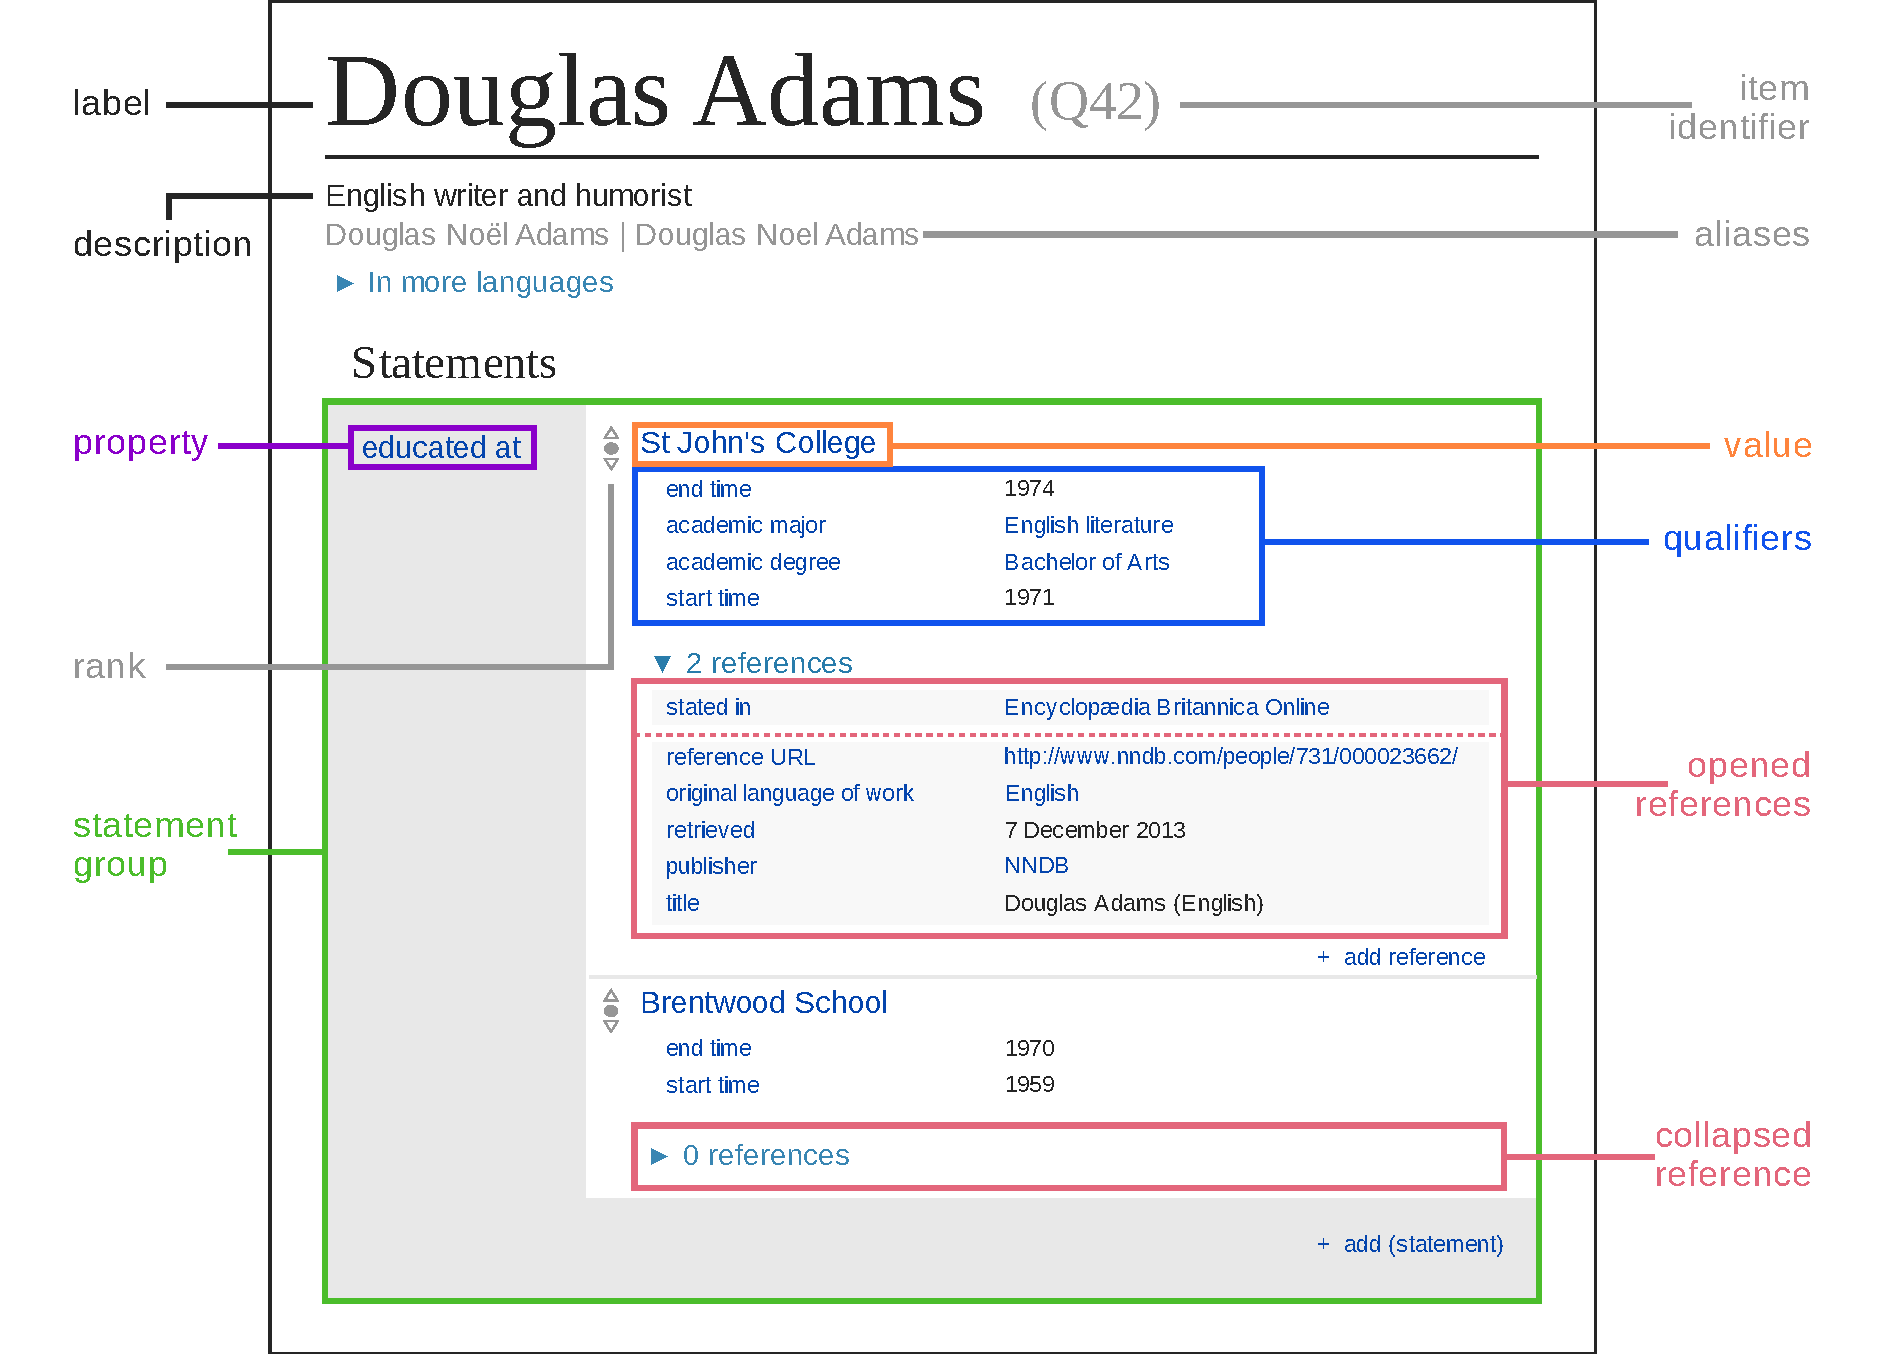
\includegraphics[width=\linewidth]{pics/Datamodel_in_Wikidata}
  \caption{Wikidata Item ``Q42''}
  \label{fig:wd-datamodel}
\end{figure}

\section{RDF}

\section{Darstellung von Wikidata als RDF}